\documentclass[12pt,a4paper]{article}

% --- Pacchetti Standard ---
\usepackage[utf8]{inputenc}
\usepackage[italian]{babel}
\usepackage{graphicx}
\usepackage{geometry}
\usepackage{hyperref}
\usepackage{booktabs}
\usepackage{listings} % Per il codice
\usepackage{fancyhdr}
\geometry{
    a4paper,
    margin=2.5cm,
    headheight=15pt, % Risolve il warning di fancyhdr (arrotondato per sicurezza)
    top=3cm          % Aumentiamo un po' il margine superiore per far spazio all'header
}
\pagestyle{fancy}
\fancyhf{} % Pulisce header e footer predefiniti

% --- Configurazione Link ---
\hypersetup{
    colorlinks=true,
    linkcolor=blue,
    urlcolor=cyan,
}

% --- Configurazione Header ---
\fancyhead[L]{F1 Fan Club} % Sinistra
\fancyhead[R]{UniPD} % Destra

% --- Configurazione Footer ---
\fancyfoot[L]{Informatica} % Sinistra
\fancyfoot[R]{Pag. \thepage} % Destra

\renewcommand{\headrulewidth}{0.4pt} % Linea sotto l'header
\renewcommand{\footrulewidth}{0.4pt} % Linea sopra il footer

\begin{document}

% --- Frontespizio ---
\begin{titlepage}
    \centering
    % LOGO UNIPD
    \begin{figure}[h]
        \centering
        
\includegraphics[width=0.25\textwidth]{../resources/logo_unipd.png} % Sostituisci con il nome corretto
    \end{figure}
    
    \vspace{0.5cm}
    {\Large \textbf{Università degli Studi di Padova}} \\
    {\large Corso di Laurea in Informatica} \\
    
    \vspace{1.5cm}
    
    % LOGO PROGETTO
    \begin{figure}[h]
        \centering
        
\includegraphics[width=0.4\textwidth]{../resources/logo.jpeg}
    \end{figure}
    
    {\Huge \textbf{F1 Fan Club}} \\
    \vspace{0.5cm}
    {\large Relazione per il progetto di Tecnologie Web} \\
    
    \vfill
    Sito web: AGGIUNGERE INDIRIZZO WEB\\
    Mail del referente: riccardo.graziani.1@studenti.unipd.it
    \vfill
    \begin{table}[h]
        \centering
        \begin{tabular}{lll}
            \textbf{Tipo di utente} & \textbf{Username} & \textbf{Password} \\ \midrule
            Utente amministratore     & admin & admin \\
            Utente semplice      & user & user \\
        \end{tabular}
    \end{table}
    \vfill
    {\large Anno Accademico 2025/2026}
\end{titlepage}

\tableofcontents
\newpage


% --- Sezioni Contenuto ---

\section{Introduzione}
Descrizione del progetto "F1 Fan Club". Obiettivi del sito, target di utenza (appassionati di motori) e finalità comunicative.

La seguente relazione serve ad illustrare la progettazione e lo sviluppo del sito web F1 FAN CLUB da parte di cinque studenti del corso di laurea di Informatica per il corso di Tecnologie Web nell'anno accademico 2025/2026. Il gruppo è formato dai seguenti studenti:

\begin{table}[h]
        \centering
        \begin{tabular}{lll}
            \textbf{Nome e Cognome} & \textbf{Matricola} & \textbf{Email (studenti.unipd.it)} \\ \midrule
            Giuliano Banchieri     & 2101081 & giuliano.banchieri@studenti.unipd.it \\
            Alessandro Frison      & 2111932 & alessandro.frison.13@studenti.unipd.it \\
            Riccardo Graziani      & 2101054 & riccardo.graziani.1@studenti.unipd.it \\
            Chiara Grossele        & 2101063 & chiara.grossele@studenti.unipd.it \\
            Mattia Oliva Medin     & 2103471 & mattia.olivamedin@studenti.unipd.it \\
        \end{tabular}
    \end{table}

Il gruppo ha deciso di sviluppare un sito fan club della Formula 1 in cui sono presenti le informazioni relative al mondo delle gare automobilistiche. Il sito è progettato per permettere agli utenti già informati su questa tematica di trovare velocemente le informazioni di cui hanno bisognro e allo stesso tempo permette ai meno esperti di imparare cose nuove relative al mondo della F1.

\newpage

\section{Analisi dei Requisiti}
Innanzi a tutto abbiamo analizzato diversi siti web relativi alla Formula 1 per capire quali funzionalità fossero più utili e interessanti per gli utenti. Abbiamo inoltre discusso tra di noi per definire le funzionalità principali del sito e le caratteristiche che volevamo implementare.
Il nostro obiettivo principale era quello di creare un sito web che fosse facile da usare, accessibile e che fornisse informazioni accurate e aggiornate sul mondo della Formula 1. 
Abbiamo inoltre prestato una particolare attenzione alla vista mobile del sito, per garantire una buona esperienza di navigazione anche su dispositivi mobili.
\subsection{Target di utenza}
F1 Fan Club è rivolto principalmente agli appassionati di Formula 1 che vogliono condividere la loro passione, sia a coloro che seguono regolarmente le gare sia a chi è interessato a conoscere meglio questo sport. Il sito è progettato per essere accessibile a un pubblico ampio, includendo sia utenti esperti che principianti.
Inoltre il nostro sito è pensato per essere utilizzato da utenti di tutte le età, con un'interfaccia intuitiva e facile da navigare, in particolare il sito si rivolge ad un'utenza con età compresa tra i 16 e i 65 anni.

\subsection{SEO}
Per migliorare la visibilità del sito sui motori di ricerca, sono state adottate le seguenti strategie SEO:
\begin{itemize}
    \item Ogni pagina è provvista di tag "title" che descrivono accuratamente il contenuto della pagina dal particolare al generale;
    \item Vengono utilizzate parole chiave pertinenti nel contenuto del sito, come "Formula 1", "piloti", "scuderie", "classifica", "gare" e "circuiti";
    \item Tutte le pagine hanno meta tag descrittivi per ogni pagina del sito, includendo le parole chiave principali;
    \item In tutte le parti del sito è stata prevista la separazione tra contenuto e presentazione, utilizzando CSS per lo stile e HTML per la struttura;
    \item Tutto il sito è soggetto alla separazione tra contenuto e comportamento, utilizzando JavaScript per le funzionalità interattive e PHP per la logica di backend; 
\end{itemize}

In particolare F1 Fan Club vuole rispondere alle seguenti query di ricerca:
\begin{itemize}
    \item "Fan Club Formula 1" o simili;
    \item qualsiasi contenga nomi di scuderie o piloti di F1 presenti nel sito;
    \item qualsiasi contenga nomi di gare o circuiti di F1 presenti nel sito;
    \item qualsiasi contenga termini relativi alla classifica di F1;
    \item qualsiasi contenga commenti o opinioni su gare di F1;
\end{itemize}

\section{Progettazione}
\subsection{Schema organizzativo}
Abbiamo adottato un approccio di progettazione dando priorità alla facilità di comprensione dei contenuti, con particolare attenzione all'usabilità e all'accessibilità. 
Il sito permette di visualizzare diverse informazioni riguardanti il mondo della Formula 1 come i piloti, le scuderie, la classifica sia dei piloti che delle scuderie, le varie gare effettuate e la lista di circuiti.
Gli utenti registrati possono inoltre commentare le varie gare, esprimendo le proprie opinioni e interagendo con altri appassionati. L'amministratore del sito ha la possibilità di gestire gli utenti, aggiungendone di nuovi o rimuovendo account in caso di commenti inappropriati,
L'amministratore potrà inoltre aggiungere o rimuovere le gare quando queste vengono effettuate utilizzando qualunque circuito disponibile, inoltre dovrà anche occuparsi di aggiornare la classifica aggiungendo o rimuovendo punti ai diversi piloti.
\subsection{Tipi di utente}
Durante la fase di progettazione sono stati identificati di seguenti tipi di utente:
\begin{itemize}
    \item \textbf{Utente non registrato:} Può visualizzare le informazioni generali sul sito, i piloti, le scuderie, le classifiche, le gare ed i circuiti, ma non può commentare diverse gare o accedere all'area riservata.
    \item \textbf{Utente registrato:} L'utente registrato può accedere a tutte le funzionalità del sito, inclusa la possibilità di commentare le gare e accedere alla propria area riservata dove potrà modificare le diverse informazioni riguardanti il suo account.
    \item \textbf{Amministratore:} L'utente amministratore ha accesso a tutte le funzionalità del sito e può inoltre aggiungere o rimuovere utenti, eliminando i commenti del'utente rimosso, potrà anche aggiungere nuove gare o rimuovere gare esistenti e potrà infine aggiornare le classifiche aggiungendo o rimuovendo punti ai diversi piloti.
\end{itemize}
\subsection{Funzionalità}
Elenco delle funzionalità del sito:
\begin{itemize}
    \item Registrazione utente;
    \item login utente/amministratore;
    \item visualizzazione home page;
    \item visualizzazione piloti;
    \item visualizzazione informazioni pilota;
    \item visualizzazione scuderie;
    \item visualizzazione informazioni scuderia;
    \item visualizzazione classifica piloti;
    \item visualizzazione classifica costruttori;
    \item visualizzazione gare effettuate;
    \item visualizzazione commenti gara;
    \item visualizzazione circuiti;
    \item inserimento commenti (utente registrato);
    \item rimozione propri commenti (utente registrato);
    \item accesso all'area riservata (utente registrato);
    \item modifica informazioni account (utente registrato);
    \item visualizzare propri commenti (utente registrato);
    \item aggiunta utenti (amministratore);
    \item rimozione utenti e relativi commenti (amministratore);
    \item aggiunta gare (amministratore);
    \item rimozione gare (amministratore);
    \item aggiunta punti al pilota nella classifica (amministratore);
    \item rimozione punti al pilota nella classifica (amministratore).
\end{itemize}
\subsection{Convenzioni interne}
Elenco delle convenzioni interne del sito:
\begin{itemize}
    \item i \textbf{link} sono tutti sottolineati. I link non visitati sono di colore bianco, mentre i link visitati sono di colore blu, sono stati scelti questi colori per garantire un buon contrasto con lo sfondo scuro del sito;
    \item i \textbf{form} hanno uno sfondo scuro, testo di colore bianco e il pulsante di invio di colore rosso.
    \item i \textbf{link circolari} sono disabilitati e vengono mostrati sottolineati di rosso per fai capire che ci si trova in quella pagina;
\end{itemize}
\subsection{Schema del Database}
Schema relazionale del database:
\begin{figure}
    \centering
    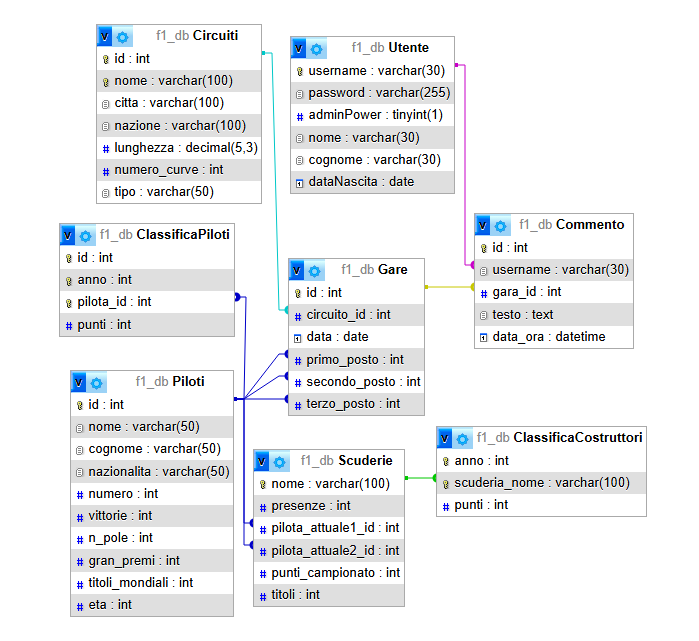
\includegraphics[width=0.8\textwidth]{../resources/databaseschema.png}
\end{figure}

\newpage

\section{Realizzazione}
Descrizione delle fasi di sviluppo, delle difficoltà incontrate e delle soluzioni adottate.
\subsection{Struttura e contenuto}
Descrizione delle pagine principali del sito e delle loro funzionalità.
\subsubsection{HTML}
\subsubsection{Popolamento database}
Per popolare il database abbiamo deciso di farlo manualmente, inserendo i dati tramite comandi SQL e senza quindi generare una grande quantità di dati. Alcuni dei dati inseriti sono dati reali ma ci sono alcune eccezioni inventate per moltre categorie.
Ad esempio sono presenti alcuni piloti inventati ed una scuderia fittizia. Le immagini dei piloti, delle scuderie e delle gare sono tutte generate tramite strumenti di intelligenza artificiale mentre le immagini dei circuiti sono immagini reali libere dal copyright.
\subsection{Presentazione}
Descrizione dell'aspetto grafico del sito, del layout e delle scelte di design.
\subsubsection{CSS}
\subsubsection{Immagini e icone}
\subsubsection{Font}
\subsubsection{Colori}
\subsection{Comportamento}
Descrizione delle funzionalità interattive del sito.
\subsection{PHP}
\subsubsection{JavaScript}
\subsubsection{Validazione dell'Input}
\subsubsection{Sicurezza}
Per quanto riguarda la sicurezza del sito, sono state adottate le diverse precauzioni:
\begin{itemize}
    \item le \textbf{query SQL} sono state realizzate utilizzando le prepared statements per prevenire attacchi di tipo SQL Injection;
    \item le \textbf{password} degli utenti presenti nel database sono state cifrate tramite l'algoritmo bcrypt per prevenire accessi non autorizzati in caso di compromissione del database, inoltre gli utenti dovranno avere precauzioni nella scelta della password, infatti dovrà avere almeno 8 caratteri tra cui almeno una lettera maiuscola, una lettera minuscola, un numero e un carattere speciale;
\end{itemize}
\subsubsection{Errori di navigazione o del server}
\subsection{Accessibilità e Usabilità}
Misure adottate per garantire l'accessibilità (es. contrasto colori, navigazione da tastiera) e l'usabilità (es. layout intuitivo, tempi di caricamento rapidi).
\subsubsection{Aiuti per lo screen reader}
\subsubsection{Compatibilità}
\subsection{Versionamento del codice}
Fin dall'inizio del progetto abbiamo utilizzato Git per il versionamento del codice sorgente. Abbiamo creato un repository su GitHub dove ogni membro del gruppo ha potuto caricare le proprie modifiche e collaborare con gli altri membri.
Questo ci ha permesso di tenere traccia delle modifiche apportate al codice, facilitando la collaborazione e la risoluzione di conflitti.
Inoltre ci ha permesso di organizzare meglio la struttura delle componenti del sito suddividendo ogni tipo di componente in sottodirectory adeguate. Questo inoltre permette di avere una chiara separazione tra i diversi linguaggi utilizzati (HTML, CSS, JavaScript, PHP) e di mantenere il codice più ordinato e facile da gestire.

\newpage

\section{Test e Validazione}
Descrizione dei test effettuati per verificare il corretto funzionamento del sito e la conformità ai requisiti iniziali.
\subsection{Navigabilità ed accessibilità}
\subsection{Falsi positivi}
A seguito dell'utilizzo di Total Validor e W3C Validator sono stati riscontranti i seguenti falsi positivi:
\begin{itemize}
    \item tutte le pagine sono soggette a segnalazioni riguardanti errori di ortografia; 
    \item molte pagine presentano errori dovuti all'inserimento di un valore [value], questo è stato fatto per sostiuire il valore tra parentesi quadre tramite php;
\end{itemize}
\subsection{Screen reader}

\newpage

\section{Suddivisione del lavoro}
Abbiamo deciso di dividerci i compiti per garantire una buona organizzazione del lavoro e per sfruttare al meglio le competenze di ogni membro del gruppo garantendo a ciascuno di implementare i diversi aspetti del sito.
Ogni membro del gruppo ha però collaborato in caso di dubbi o difficoltà durante l'implementazione delle varie funzionalità aiutandoci a vicenda.
\subsection{Divisione generale dei compiti}
\begin{itemize}
    \item Banchieri Giuliano: 
    \begin{itemize}
        \item HTML e CSS di area utente, area amministratore, classifica, home page;
        \item PHP delle stesse pagine;
        \item JS: menu;
        \item Relazione.
    \end{itemize}
    \item Frison Alessandro:
    \begin{itemize}
        \item HTML e CSS di commenti, gare, circuiti;
        \item PHP delle stesse pagine;
        \item JS: classifica, area conferma elimina;
        \item Database: creazione, query e popolamento
        \item Relazione
    \end{itemize}
    \item Graziani Riccardo: 
    \begin{itemize}
        \item HTML e CSS piloti di piloti, informazioni pilota, scuderie, informazioni scuderia;
        \item PHP delle stesse pagine;
        \item JS: validazione input;
        \item Testing;
        \item Database: connessione;
        \item Relazione.
    \end{itemize}
    \item Grossele Chiara: 
    \begin{itemize}
        \item HTML e CSS di pagine d'errore, classifica, home page;
        \item PHP delle stesse pagine;
        \item JS: animazioni;
        \item Relazione.
    \end{itemize}
    \item Oliva Medin Mattia: 
    \begin{itemize}
        \item HTML e CSS di login, registrazione, pagine dei vari form admin;
        \item PHP delle stesse pagine;
        \item JS: validazione input;
        \item Database: creazione, query e popolamento;
        \item Relazione.
    \end{itemize}
    
\end{itemize}

\newpage

\section{Note}

\end{document}